\documentclass{ximera}

\author{Wim Obbels and Bart Snapp}

\title{First steps in Ximera}

\begin{document}
\pdfOnly{\onecolumn\begin{multicols}{2}}
        \begin{abstract}
            Try out Ximera!
        \end{abstract}
        \maketitle

        To use Ximera, you must have a \link[\github]{https://github.com}
        account.
        \github\ is a web platform where developers can store, share, and
        manage
        their code. It uses \verb!git!, popular software for version control,
        to help
        teams work together simultaneously
        without overwriting each other's changes. \github\ has	issue tracking,
        pull requests for proposing changes, and other project management
        tools. It's
        like a shared folder
        for coding, designed to help teams work smarter and track progress.
        Go to \url{https://github.com} and either sign-up or log-in. Note, you
        must
        know
        your \textbf{username} and \textbf{password}, so store them in a safe
        place; like in a safe, or under your bed.

        After you have a \github\ account, log-in and go to:
        \begin{center}
            \url{https://github.com/ximeraProject/ximeraFirstSteps}
            %% 230% on my horiz screen
        \end{center}

        You will see something like this:
        \pdfOnly{\end{multicols}}
\begin{image}
    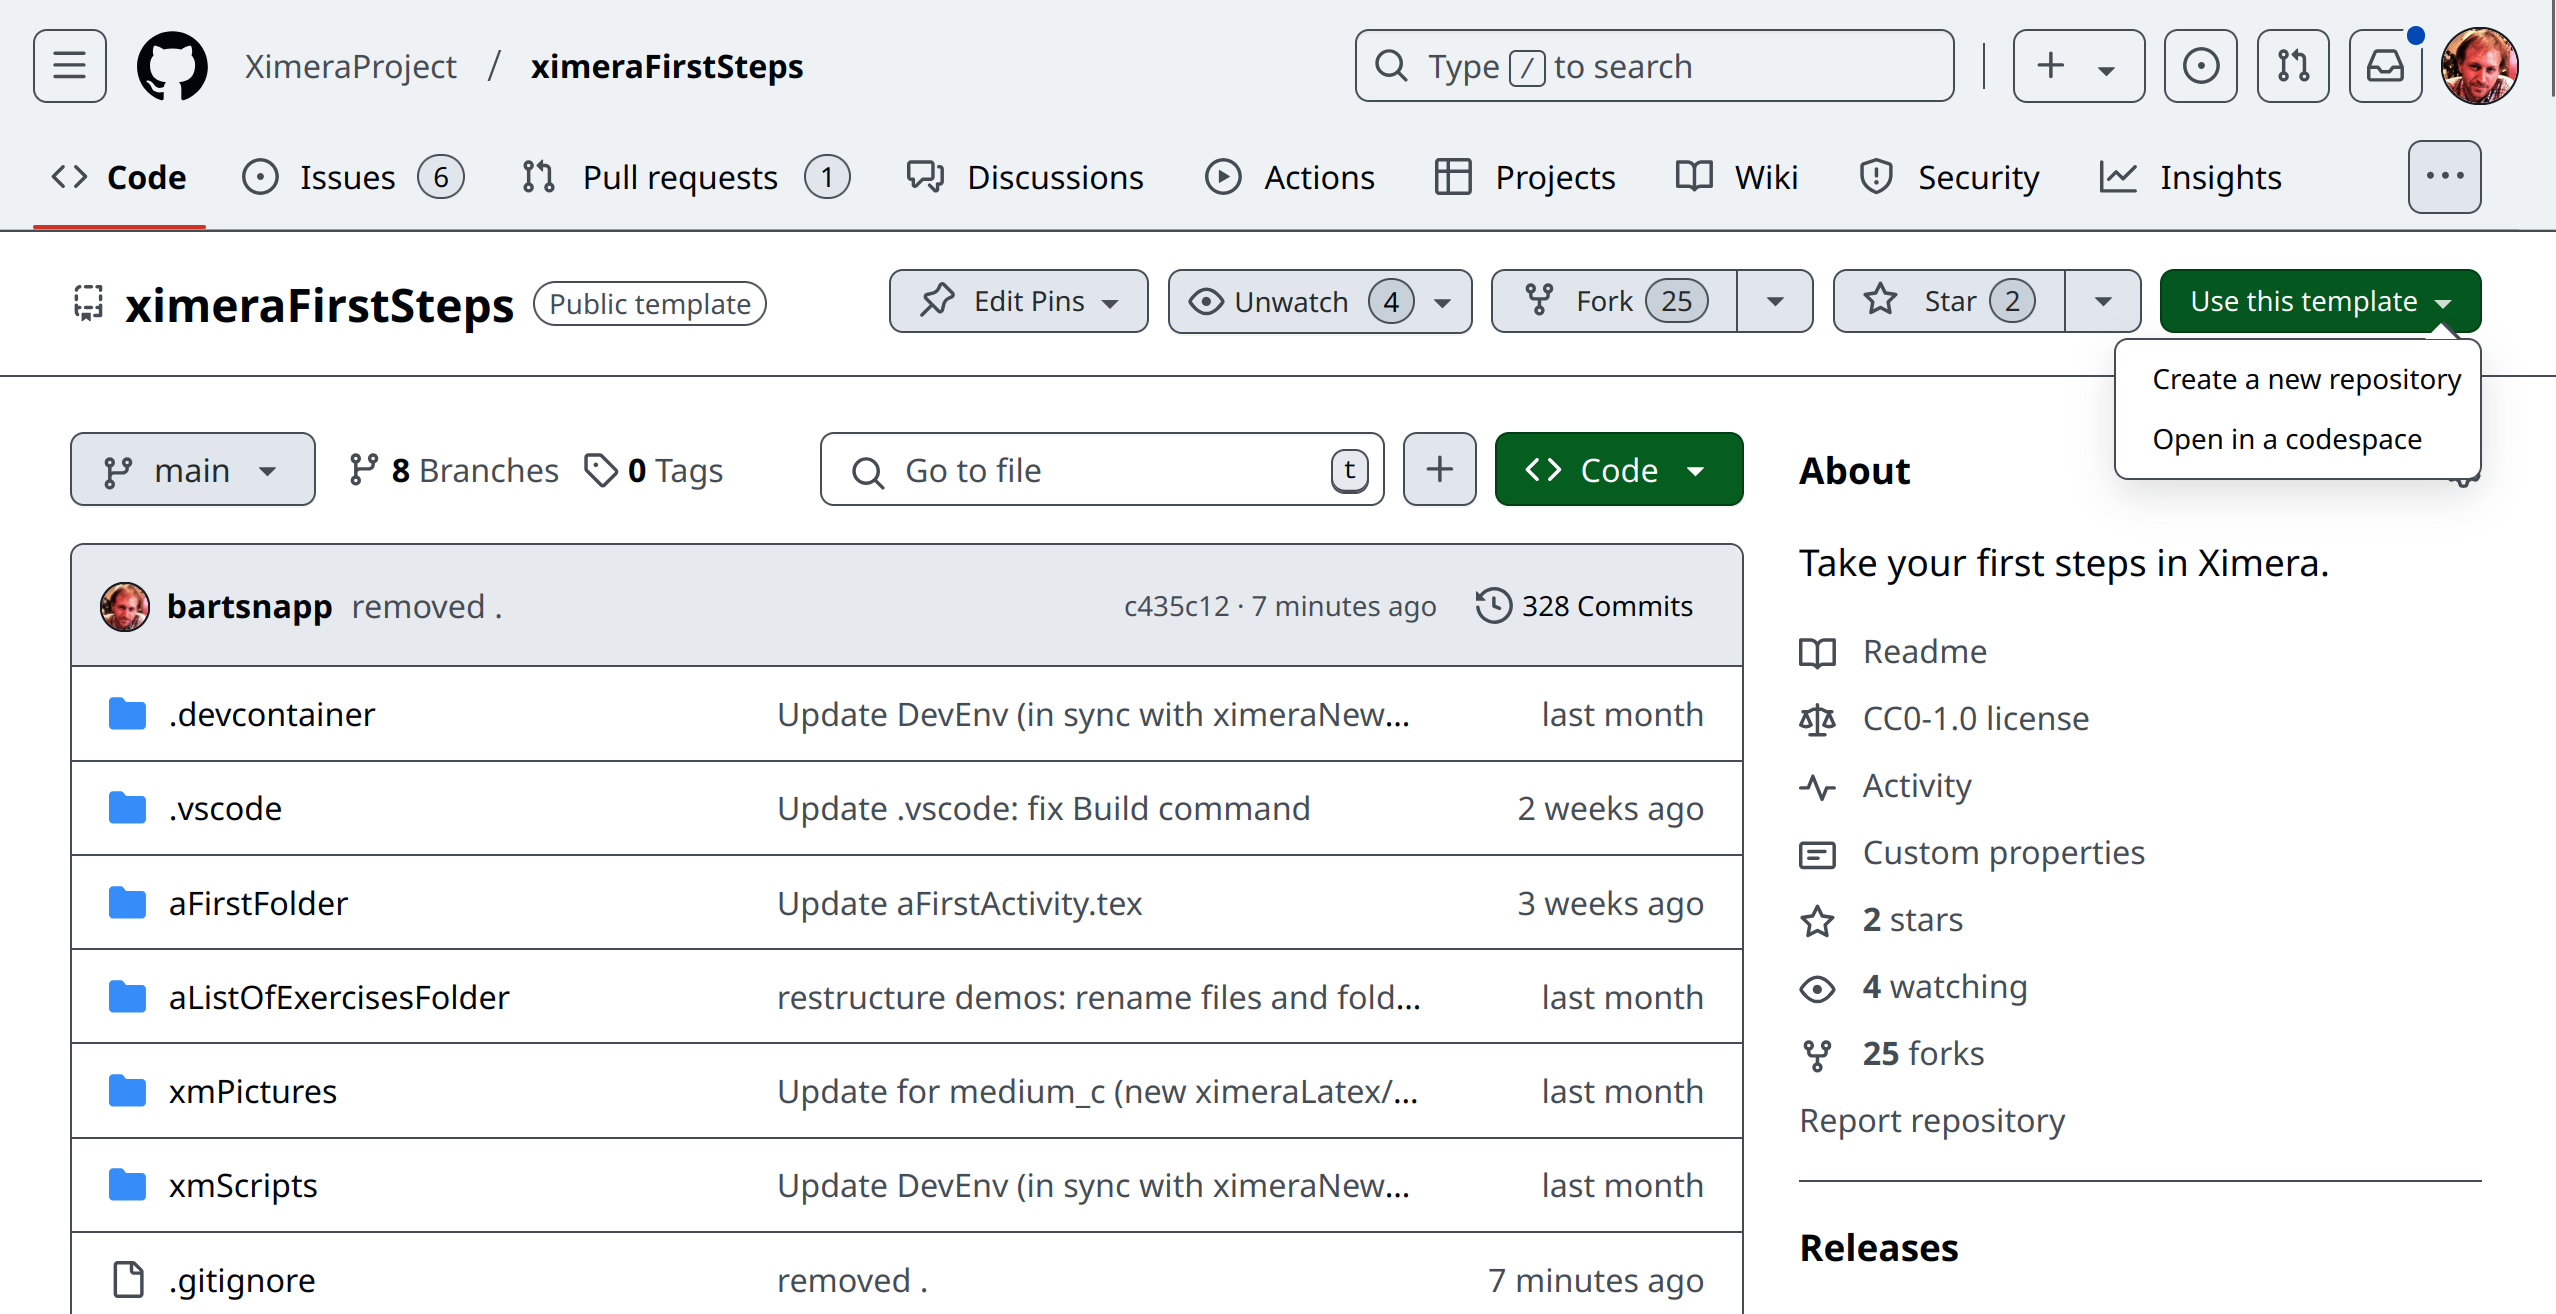
\includegraphics[width=.7\textwidth]{xfsTemplate}
\end{image}
\newpage
%\pdfOnly{\begin{multicols}{2}}
        Click on the green ``Use this template'' button and select ``Create a
        new repository.'' Give it a fun repository name, and push the button
        ``Create repository.'' 
%\pdfOnly{\end{multicols}}
\begin{image}
    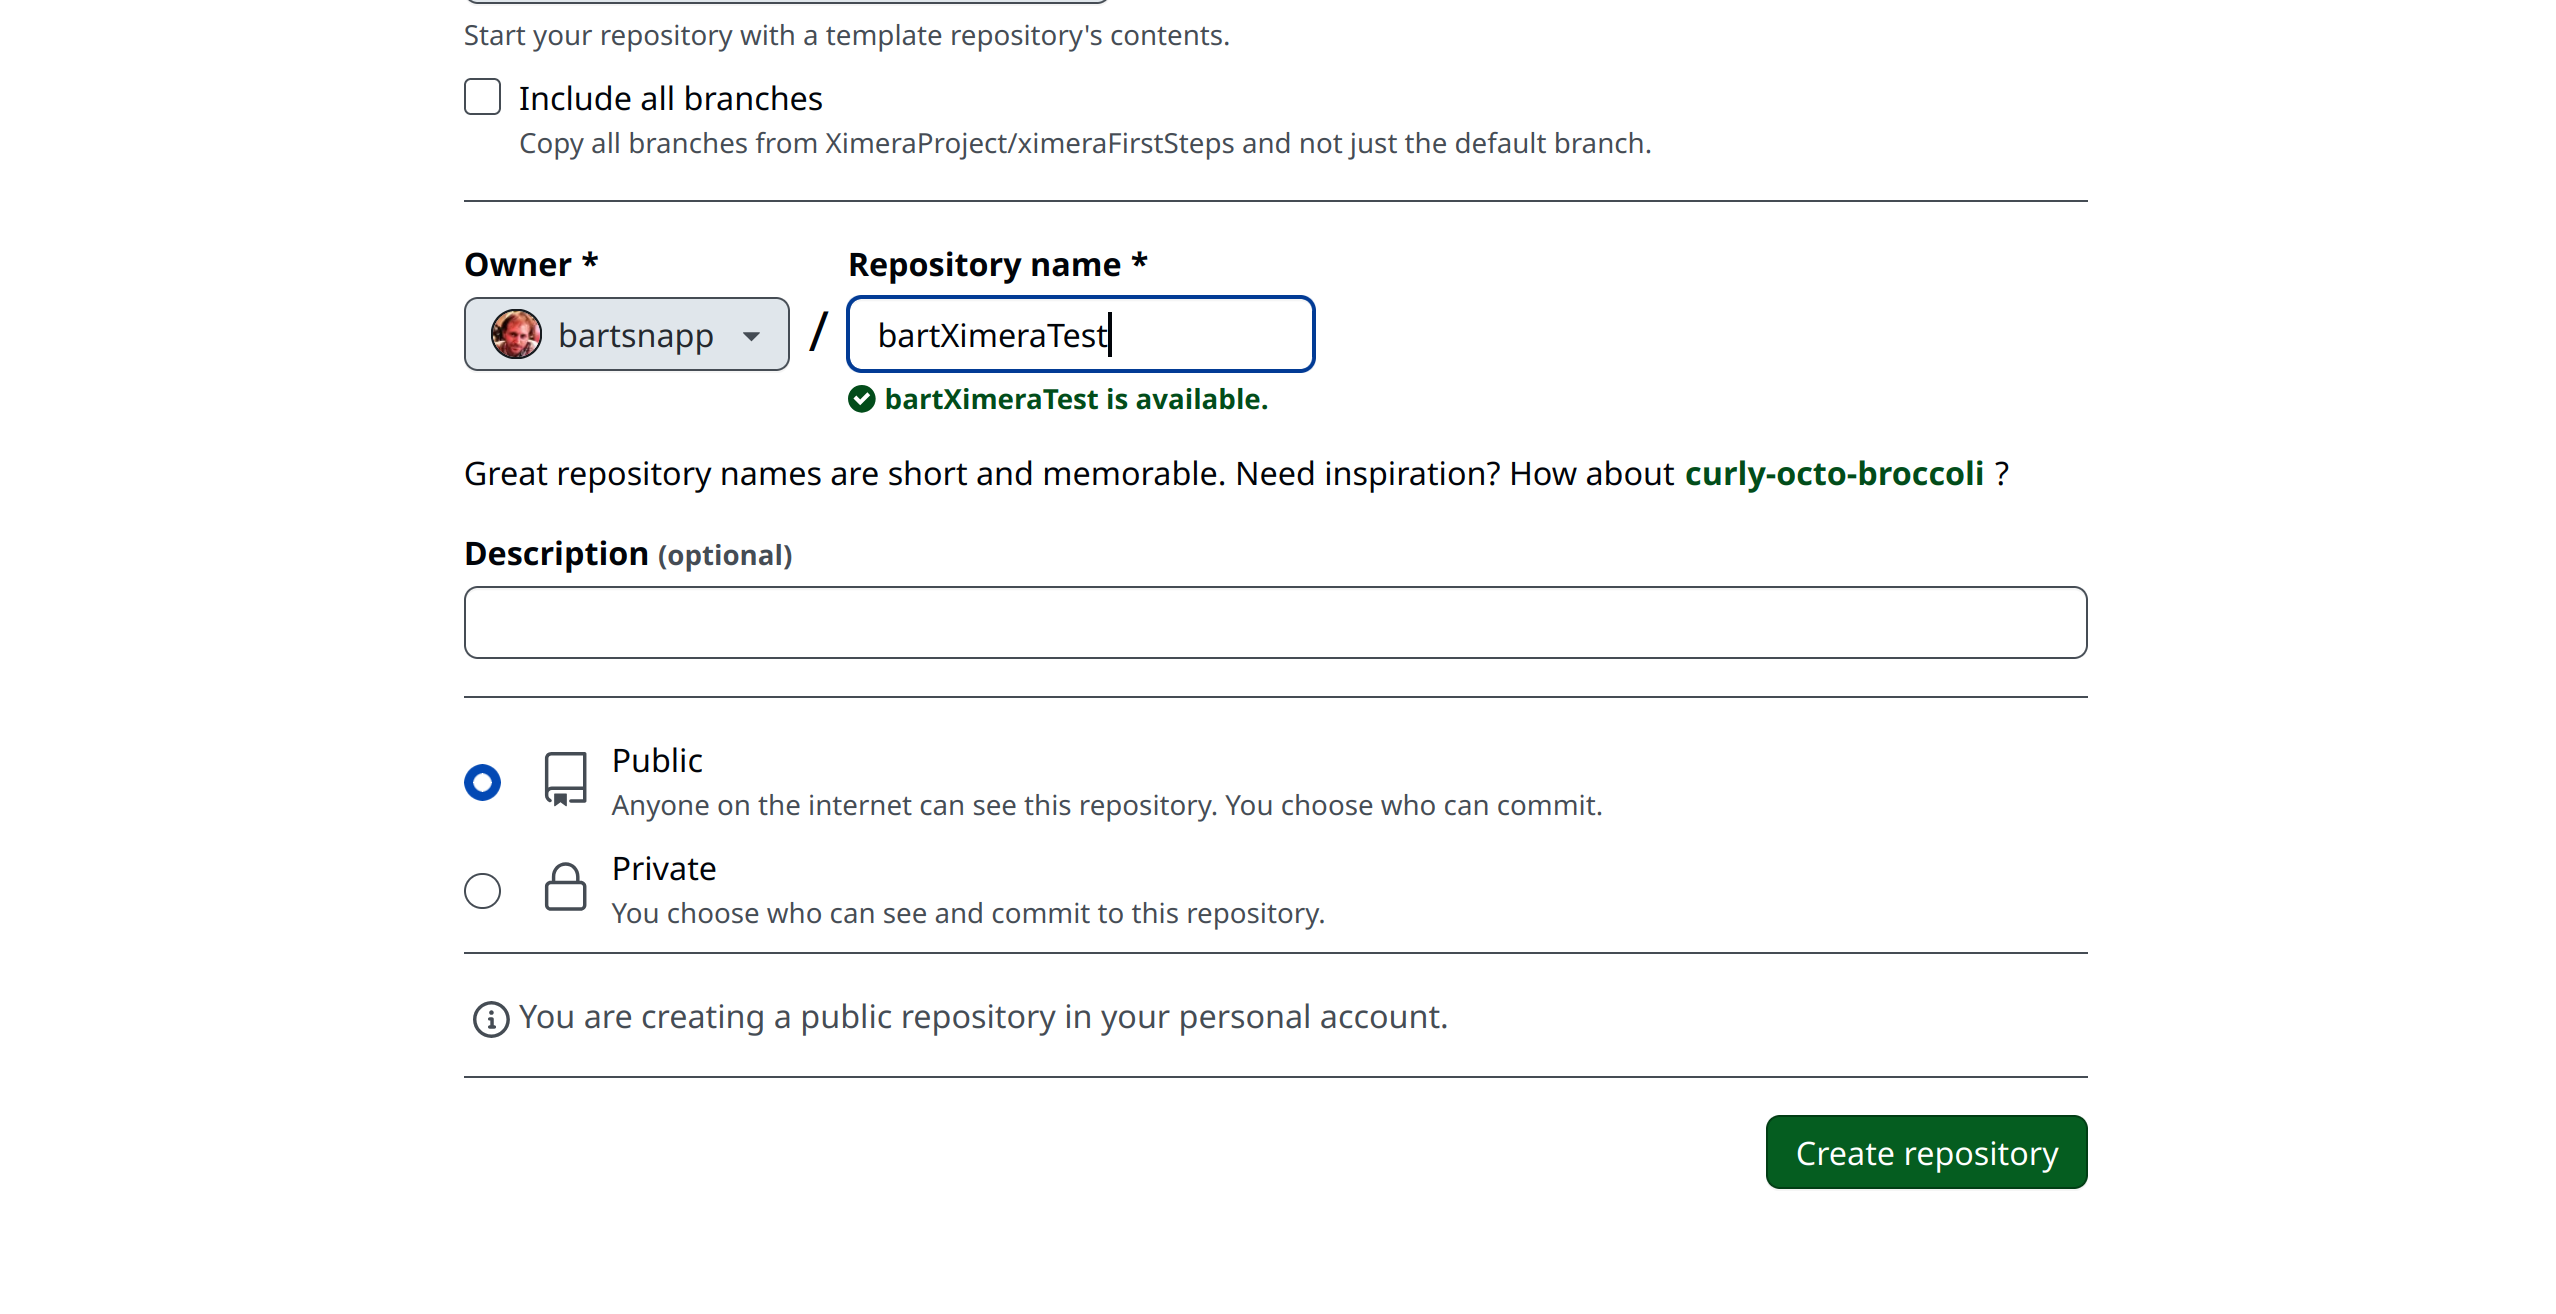
\includegraphics[width=.7\textwidth]{xfsCreate}
\end{image}
%\pdfOnly{\begin{multicols}{2}}
At this point you have your own personal copy of our repository \verb!XimeraFirstSteps!. 
In fact, after you create it, \github\ will take you to it. This copy can always be found at
\begin{center}
    \url{https://github.com/YOUR-GIT-USER-NAME/YOUR-REPO-NAME}
\end{center}
\newpage
% \pdfOnly{\end{multicols}}
\begin{image}
    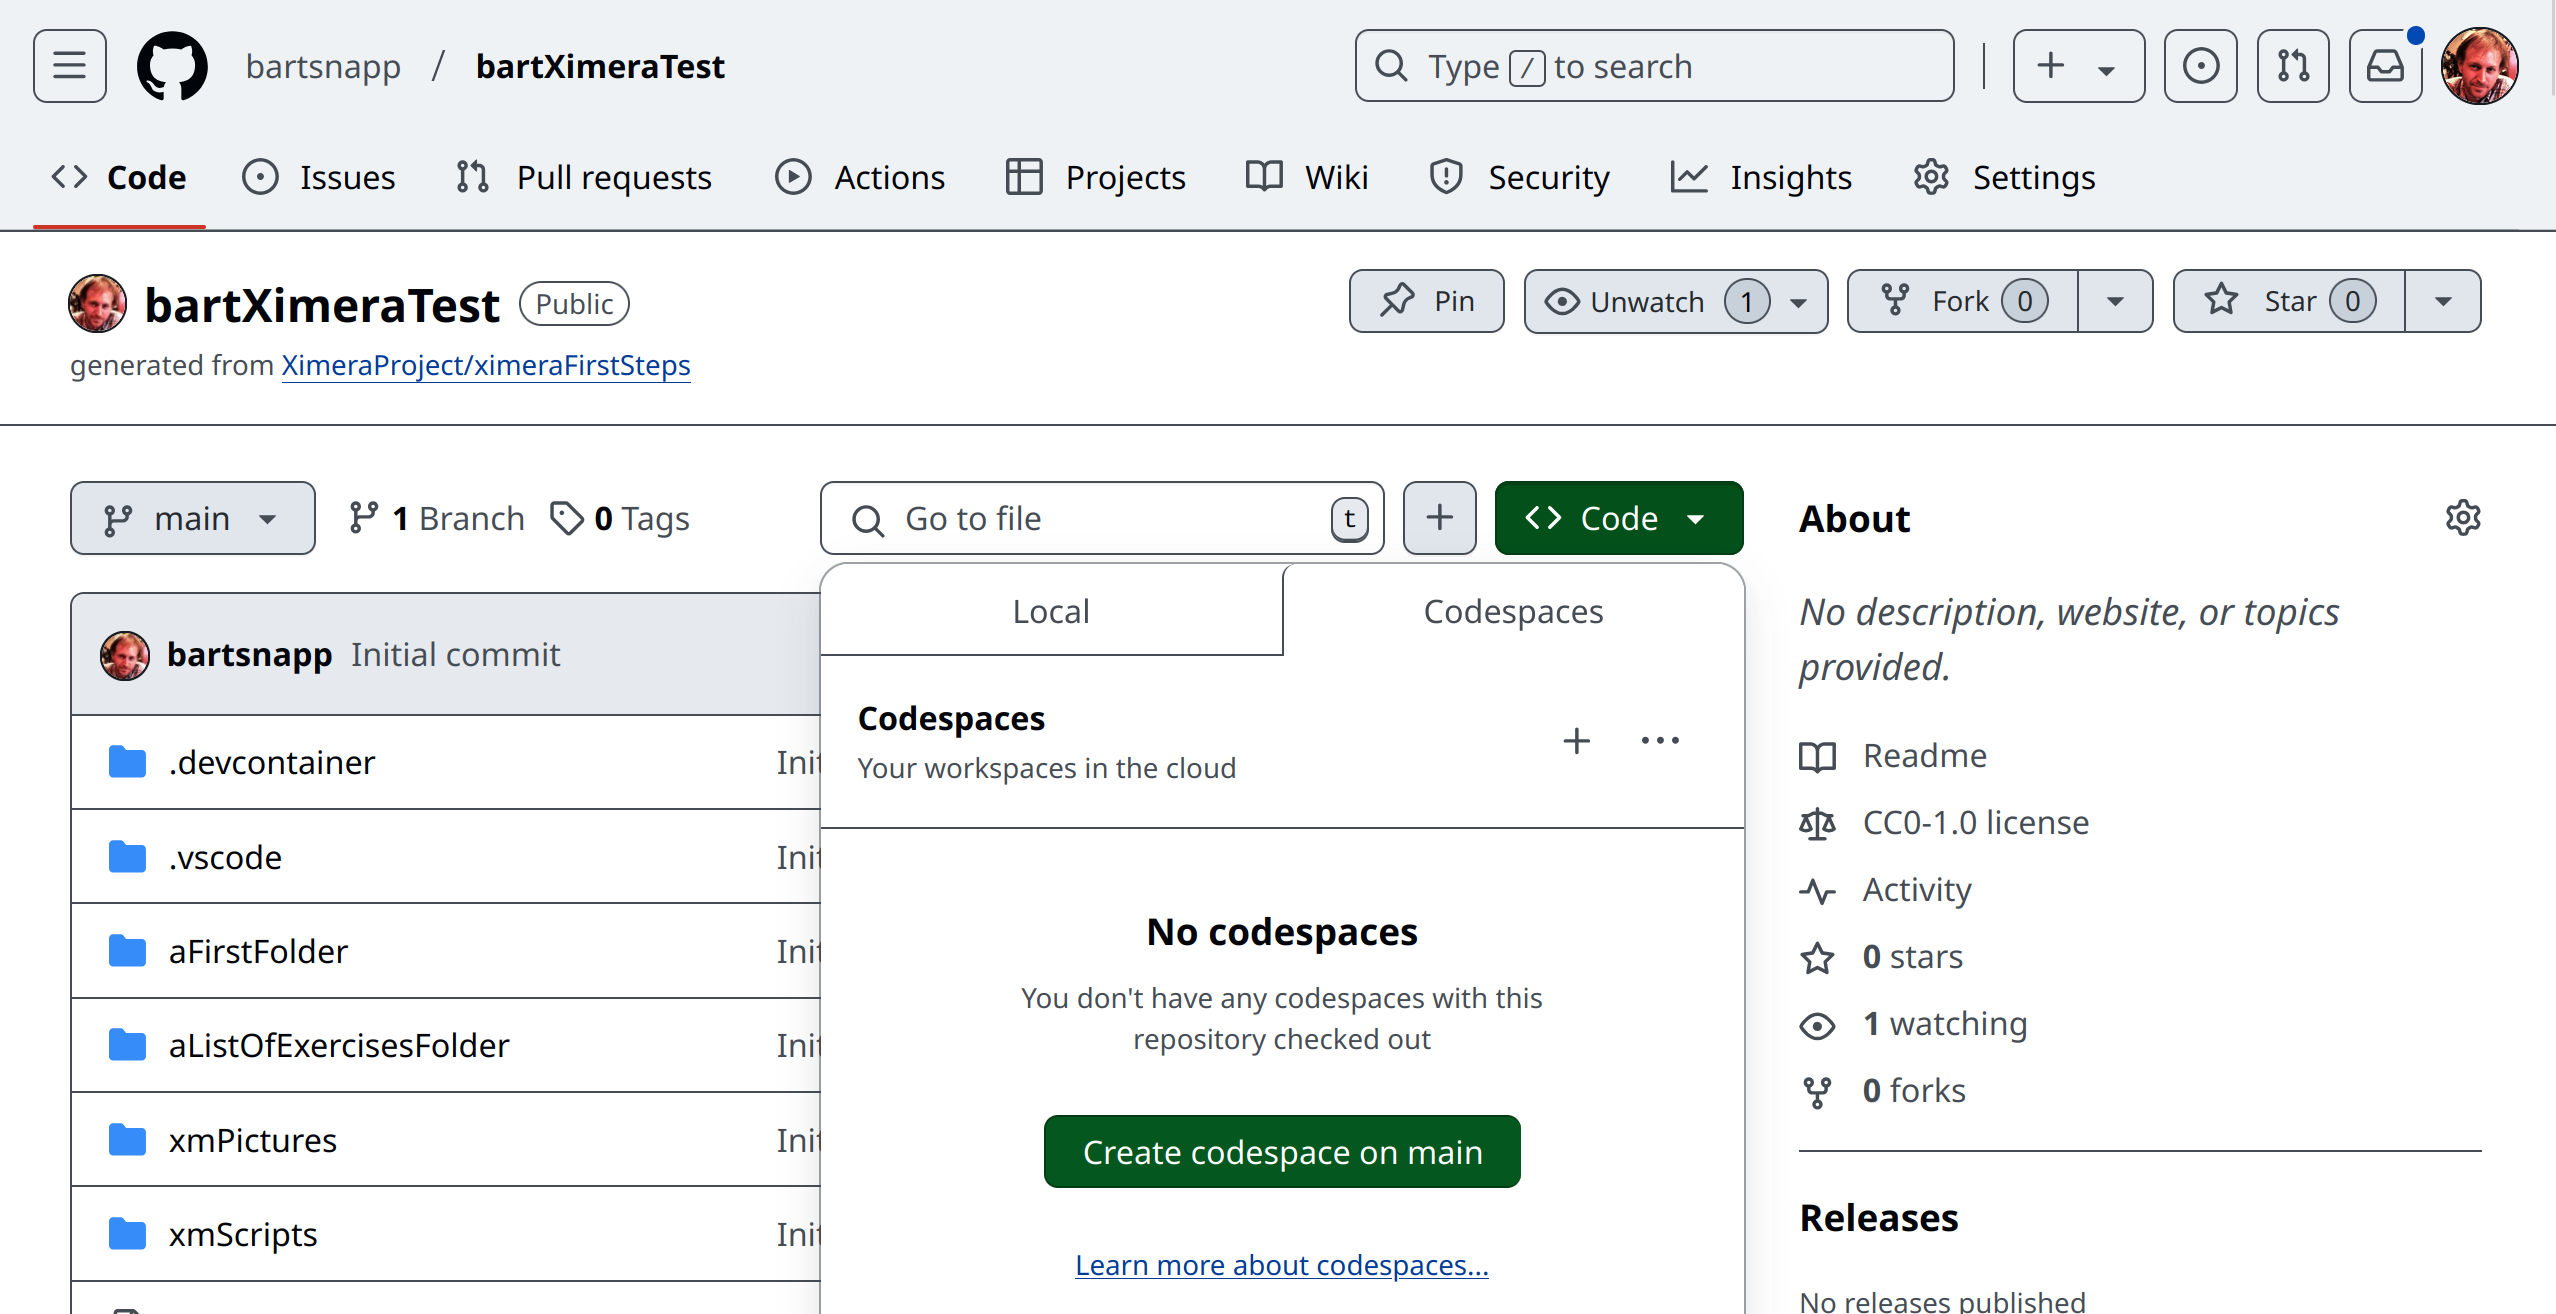
\includegraphics[width=.7\textwidth]{xfsCodespace}
\end{image}
    Once there, click the green ``code'' button, select
        the ``Codespaces'' tab, and click ``Create codespace on main.''
        A \github\ codespace is like a remote computer set up specifically for coding.
        It's a cloud-based environment where you can write, test, and run your code,
        just like on your own computer, but everything happens on remote servers. It
        comes preconfigured with all the tools, libraries, and settings you need for
        your project. You connect to it through your browser or favorite editor, and
        because it's tied to your GitHub projects, you can instantly start working
        without worrying about setting up software on your local machine. It's like
        having a ready-to-use, fully equipped coding computer that you can access from
        anywhere. \textbf{It will take around 5 minutes for your codespace to be
            created.}

\newpage

Once the codespace is created, you will see something like this:
\begin{image}
    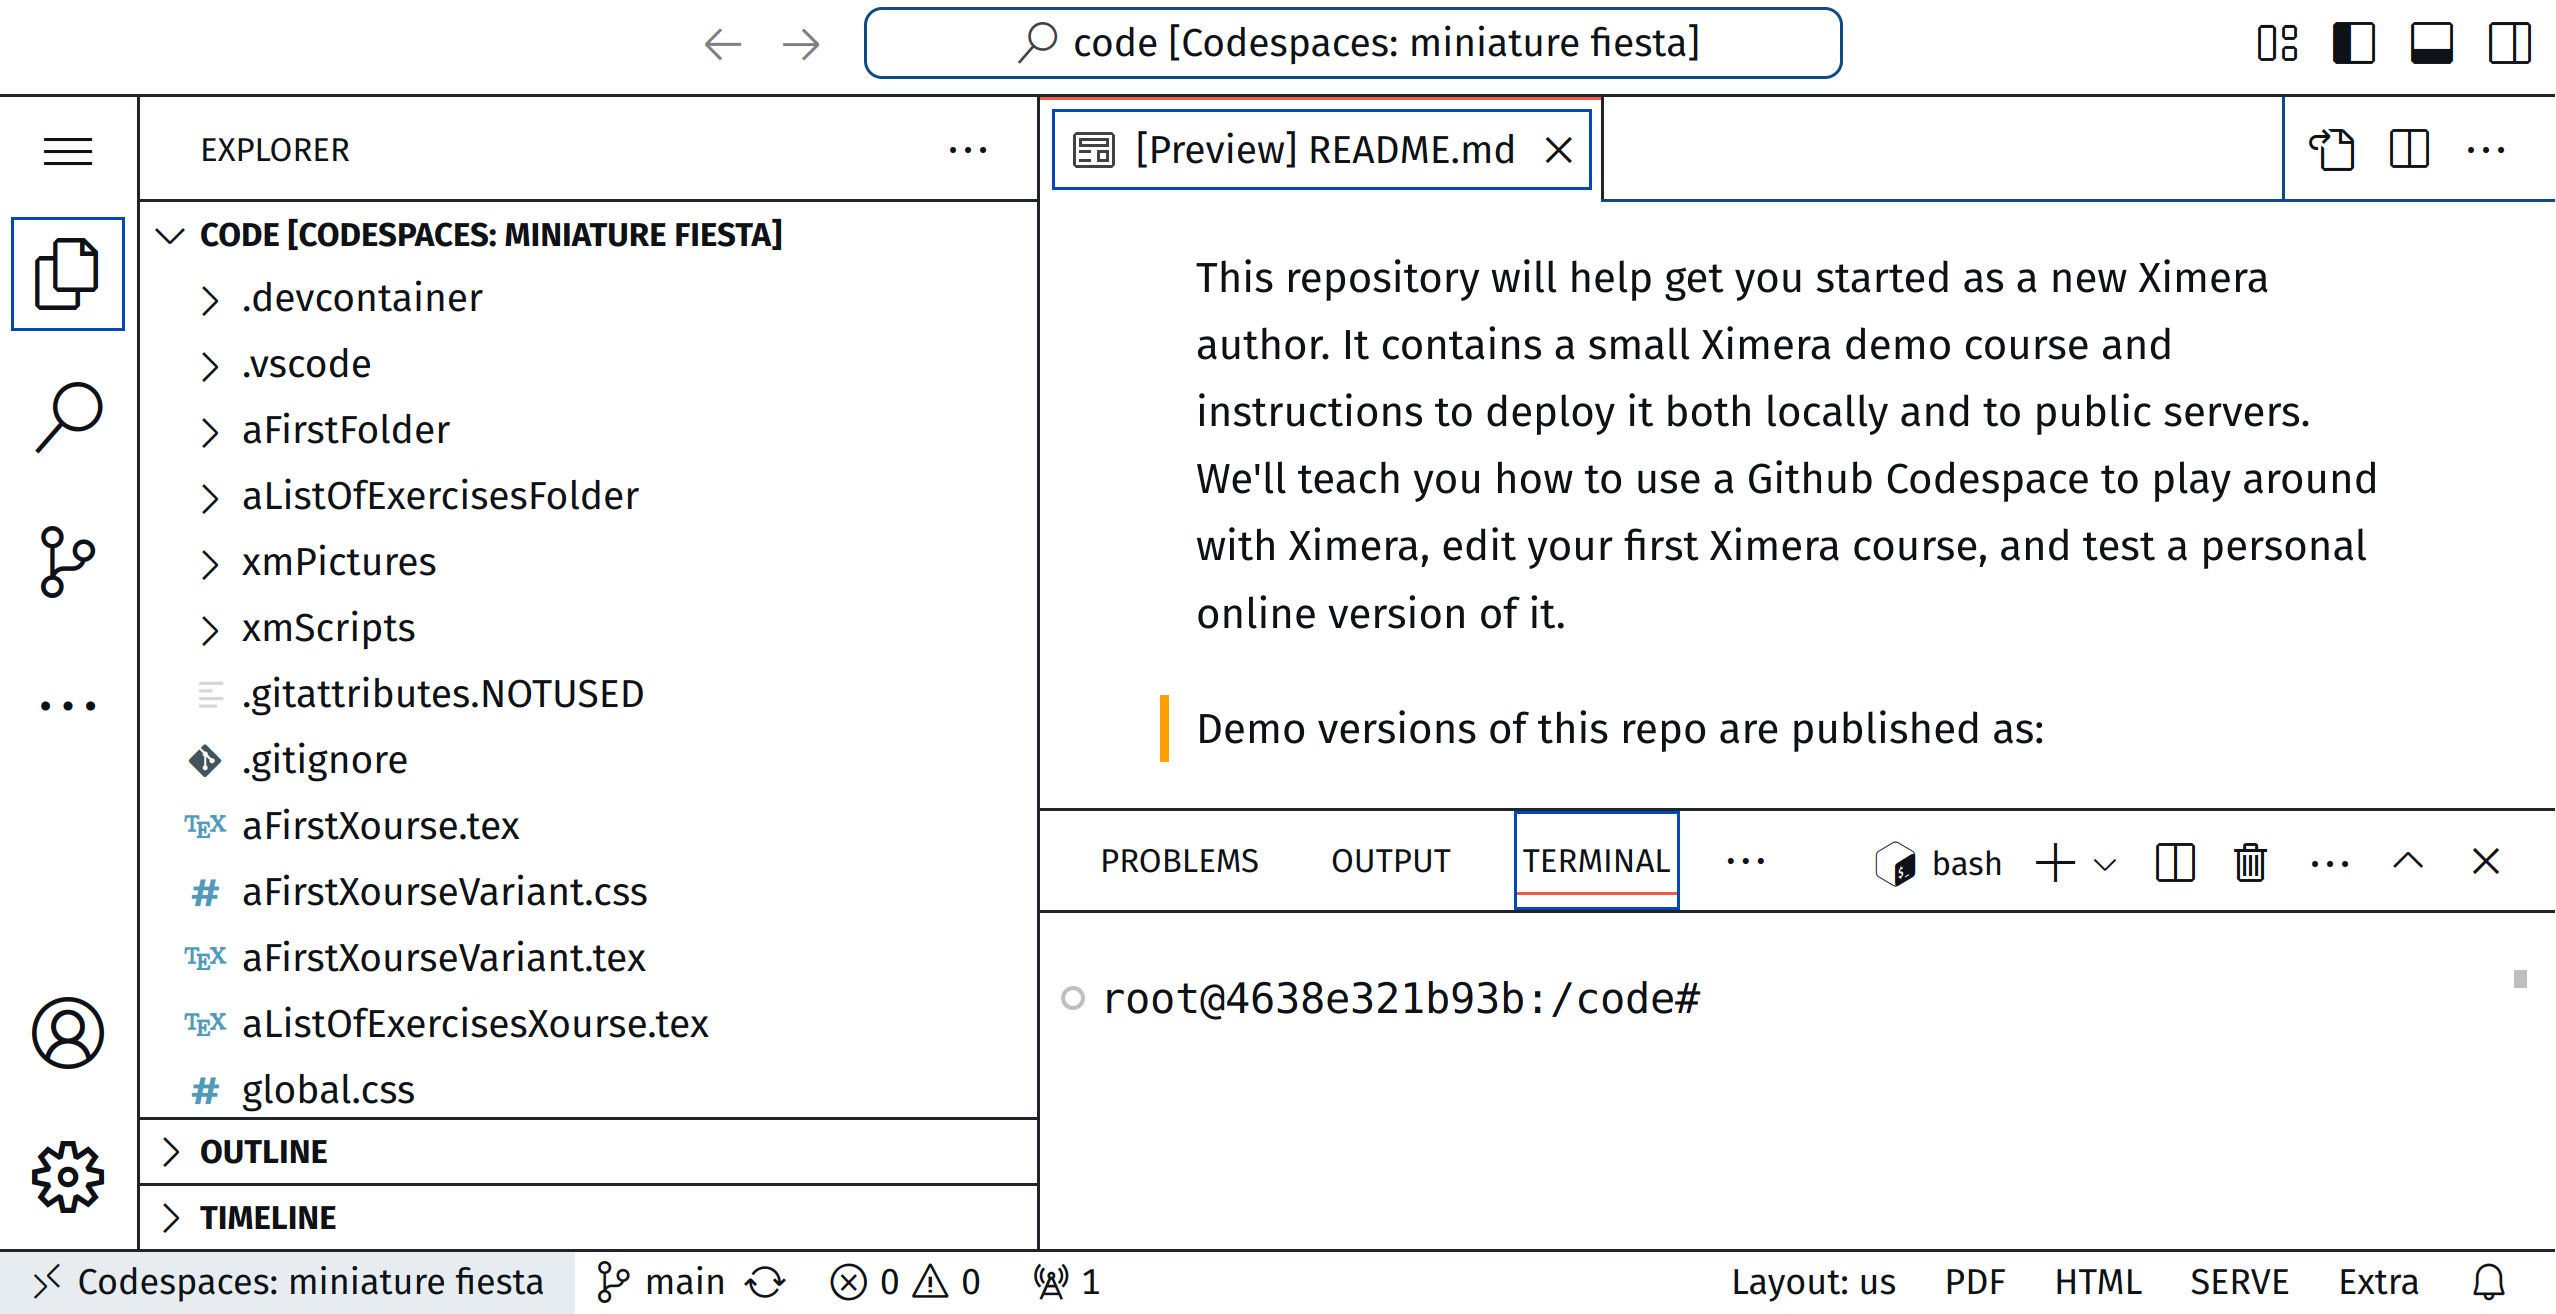
\includegraphics[width=.7\textwidth]{xfsVScode}
\end{image}

At the bottom right-hand corner of the screen you will see a button that says
``SERVE.'' Press the ``SERVE'' button to compile Ximera content to HTML and JavaScript.  This will take a few minutes.

\newpage
 Once the compilation is finished, note the line that says:
``PROBLEMS,'' ``OUTPUT,'' ``DEBUG CONSOLE,'' ``TERMINAL,'' ``PORTS.'' You want to click on ``PORTS.'' The ``PORTS'' tab may be hidden within $\cdot \cdot \cdot$.  
\begin{image}
    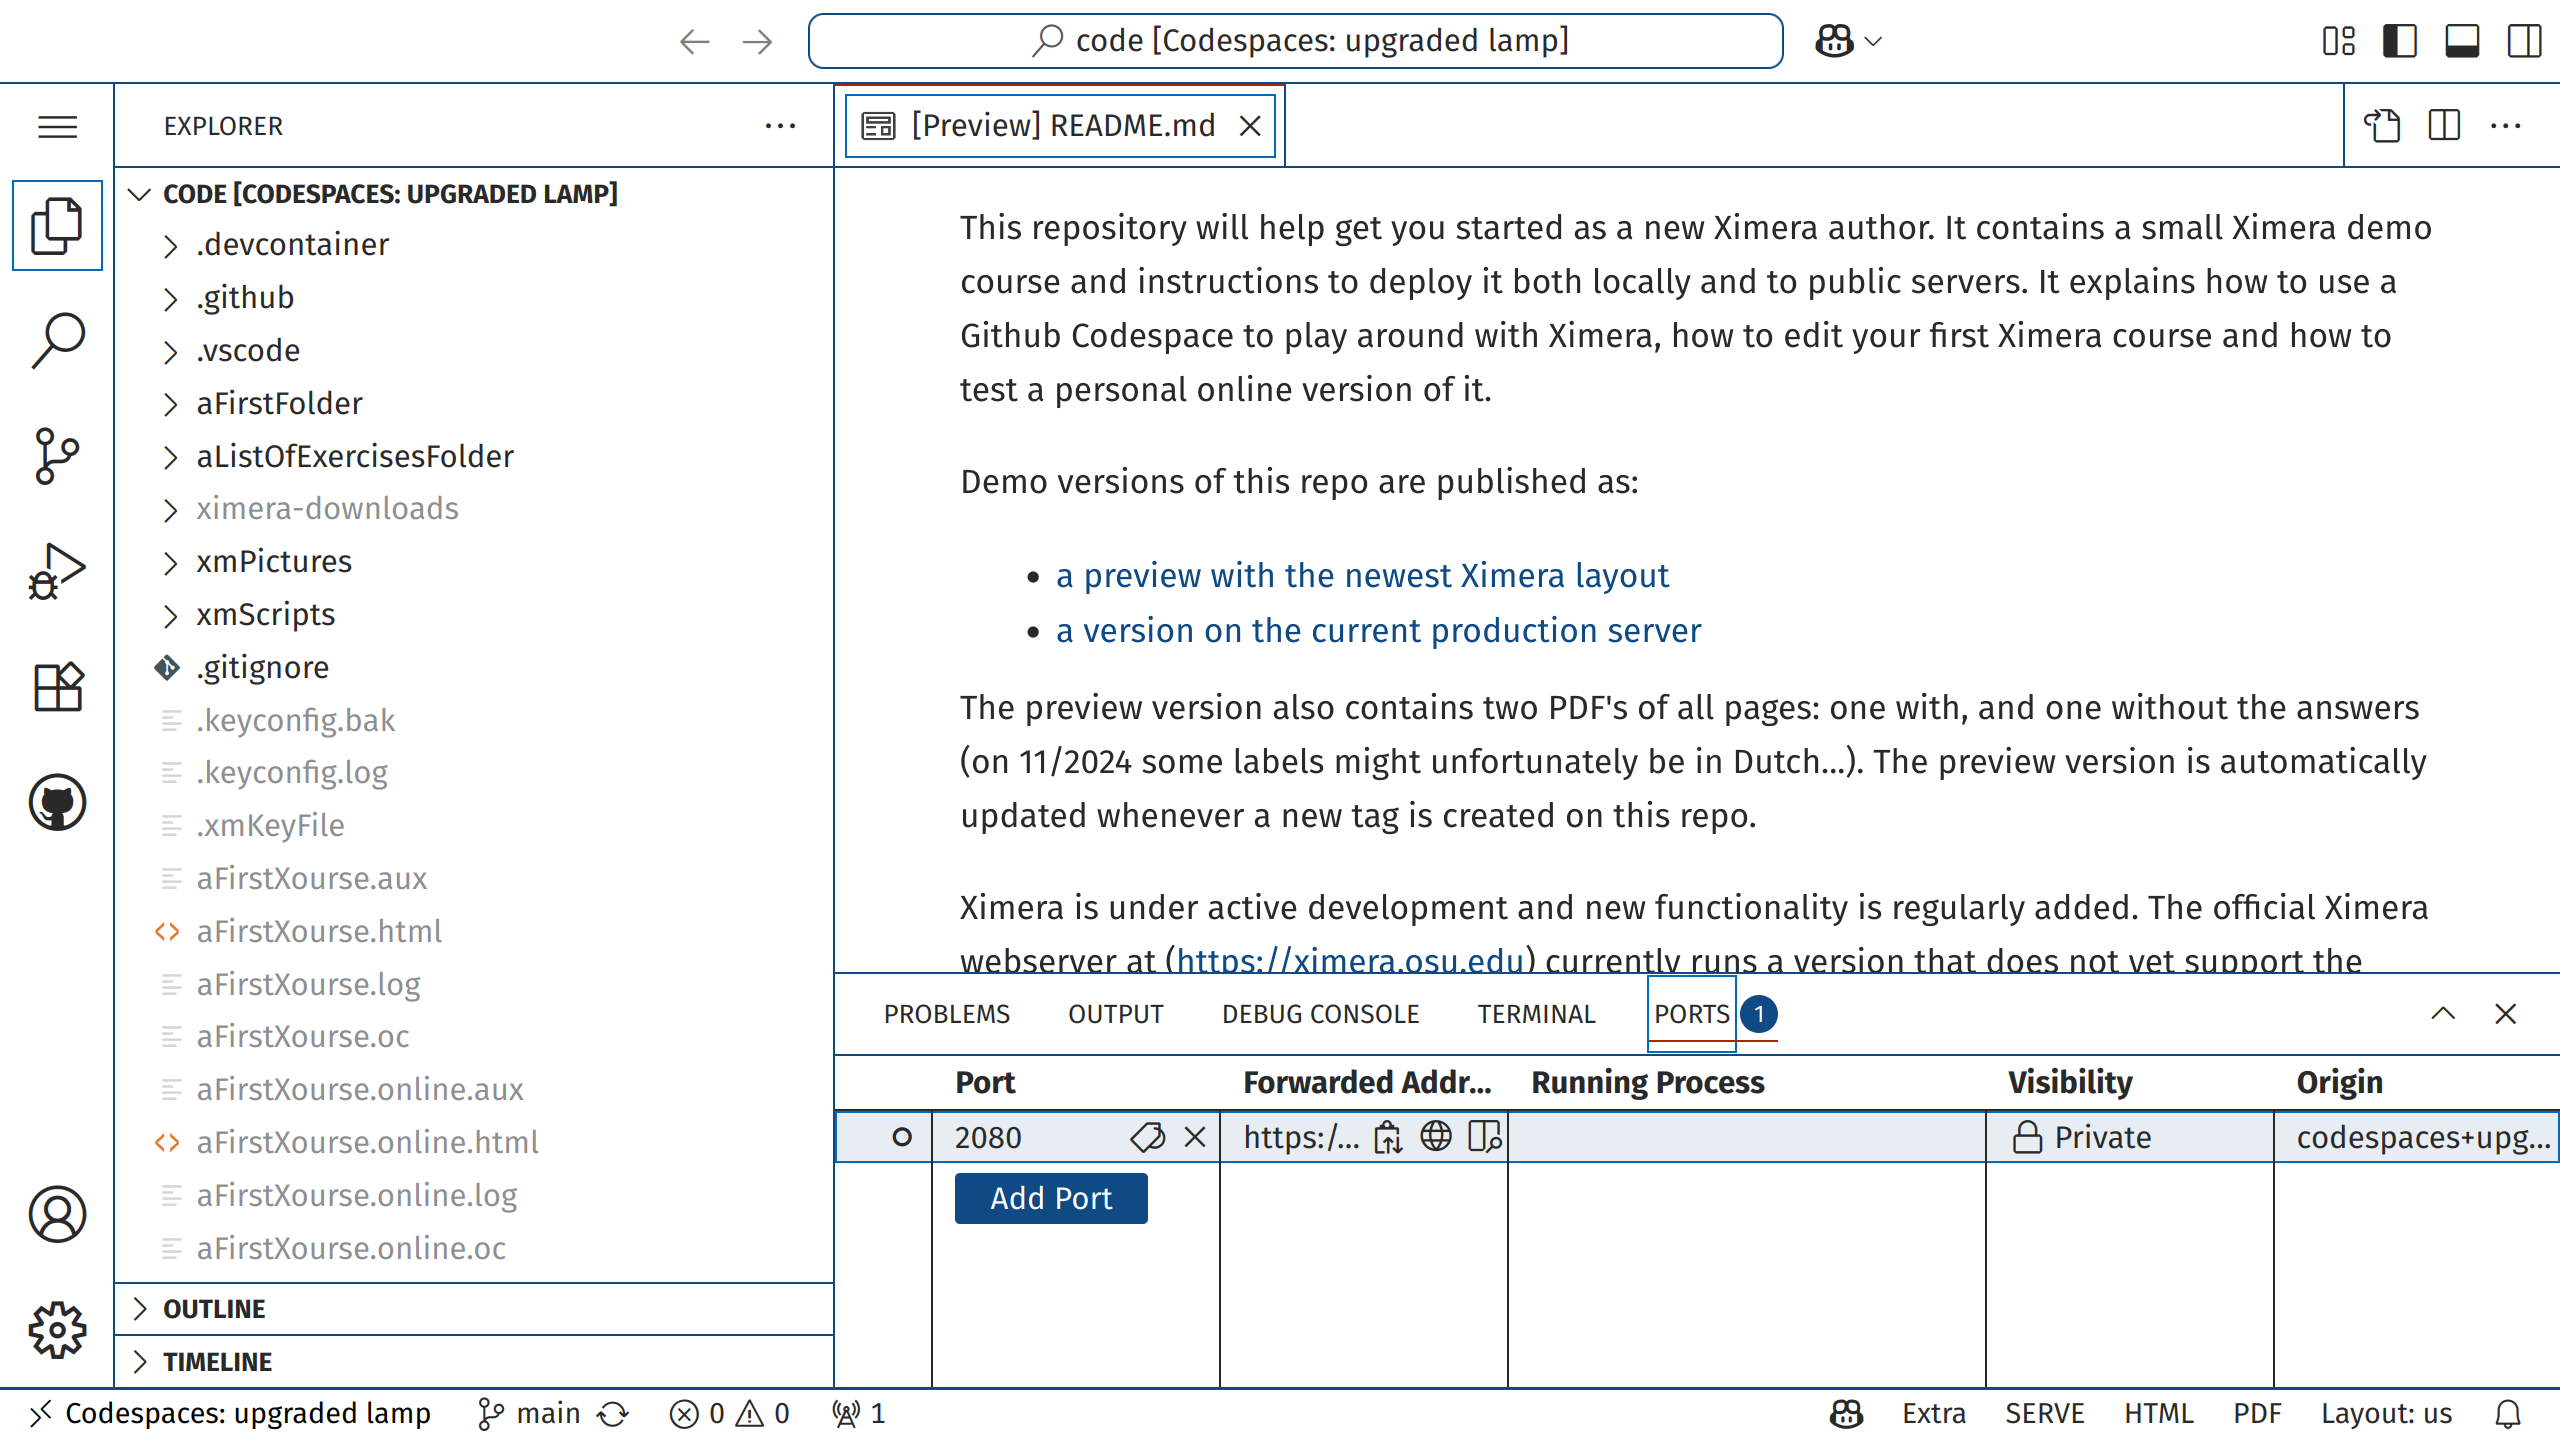
\includegraphics[width=.7\textwidth]{xfsPorts}
\end{image}
After you click on ``PORTS,'' click on the globe, and a webpage will open. Your content will be under the link ``Content.'' You should be able to see the content in your browser. 
Demo versions of this repo are published as:
\begin{itemize}
\item \link[a preview with the newest Ximera layout]{https://set.kuleuven.be/voorkennis/firststeps24/aFirstXourseVariant/aFirstFolder/aFirstActivityVariant}
\item \link[a version on the current production server]{https://ximera.osu.edu/firststeps24/aFirstXourse/aFirstFolder/aFirstActivity}
\end{itemize}
\pdfOnly{\twocolumn}
\end{document}